\chapter{The Structure of $\R^n$}

\section{Metric Space}

\begin{definition}
    Considering a set $A$, a \underline{distance function or metric} on $A$ is a function $$d: A \times A \longrightarrow \R$$
    with three properties:
    \begin{enumerate}
        \item Reflexivity: $\forall x,y \in A. d(x,y)=d(y,x)$
        \item Non-negative: $d(x,y) \geq 0 \text{ and } d(x,y)=0 \Leftrightarrow x=y$
        \item Triangle-inequality: $d(x,y) \leq d(x,z)+d(z,y)$
    \end{enumerate}
\end{definition}

\noindent \textbf{Example}:
\begin{itemize}
    \item \underline{Discrete distance}: For any set $A$
    \begin{equation}
        d(x,y)= \begin{cases}
            0 \text{ if } x=y\\
            1 \text{ if } x \neq y
        \end{cases}
    \end{equation}
\end{itemize}

\begin{definition}
    A \underline{metric space} is a set $X$ together with a specific distance function $d$ on X, we denote it as $(X,d)$.
\end{definition}

\begin{definition}
    If $(X,d)$ is a metric space, then any subset $A \subset X$ inherits a distance function $d|_A$ from $X$, 
    we call it \underline{restriction of $d$ to $A \times A$}
\end{definition}

\begin{definition}
    A \underline{ball} of radius $\epsilon$ around $a$ in $X$ with respect to any distance function $d$ is $$U(a;\epsilon)=\{x \in X: d(x,a) < \epsilon\}$$
    which is also called the \underline{$\epsilon$-neighborhood of $a$}
\end{definition}

\begin{definition}
    Let $(X,d)$ be a metric space. Let $Y \subset X$ be given, we can define the \underline{$\epsilon$-neighborhood of a set}:
    $$\epsilon\text{-neighborhood}(Y)=\bigcup_{y \in Y}U(y;\epsilon)$$
\end{definition}
\begin{figure}[ht]
    \centering
    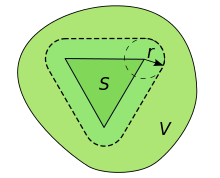
\includegraphics[scale=0.8]{images/Neighborhood_illust3.svg.png}
    \caption{r-neighborhood of the set $S$}
\end{figure}

\begin{definition}
    Let $(X,d)$ be a metric space, let $C \subset X$, we can define the \underline{distance from $x$ to $C$}:
    $$dist(x,C)=inf\{d(x,c):c \in C\}$$
\end{definition}

\begin{theorem}
    $$dist(x,C)-dist(y,C)\leq d(x,y)$$
\end{theorem}


\begin{definition}
    Let $f:(X,d_X)\longrightarrow (Y,d_Y)$. $f$ is called \underline{isometry} if it is a distance-preserving transformation between metric spaces.
    $$\forall a,b\in X.d_Y(f(a),f(b))=d_X(a,b)$$
\end{definition}

\begin{definition}
    A function $f:(X,d_X)\longrightarrow(Y,d_Y)$ is an \underline{isomorphism} if $f$ is an isometry and $f$
    is surjective. Two metric spaces are called \underline{isomorphic} if there is an isomorphism between them.
\end{definition}

\noindent \textbf{Remark}:
\begin{itemize}
    \item You can have a space that is a metric space, but not a vector space. Metric spaces do not need to have the notion of addition, or scaling. 
    \item It also can be the other way around as well. You can have a vector space that is not a metric space. Usually though we work with what are called normed vector spaces, which also have the notion of length of a vector. And these spaces induce a corresponding metric. (We talked about this in MAT247)
    \item All norms can be used to create a distance function as in $d(x,y)= \lVert x-y \rVert$, but not all distance functions have a corresponding norm.
\end{itemize}

\section{Metrics of $\R^n$}

\begin{definition}
    For the vector space $\R^n$, we can define the following norms to make different normed vector spaces. Let $x=(x_1,\cdots,x_n)\in \R^n$.
    \begin{itemize}
        \item We can define the \underline{Manhattan norm}:
        $$\lVert x \rVert_1=\sum_{j=1}^n|x_j|$$
        \item We can define the \underline{Euclidean norm}:
        $$\lVert x \rVert_2=\sqrt{\sum_{j=1}^nx_j^2}$$
        \item  We can define the \underline{Infinity norm}:
        $$\lVert x \rVert_{\infty}=sup\{|x_1|,\cdots,|x_n|\}$$
    \end{itemize}
\end{definition}


\begin{definition}
    For the vector space $\R^n$, the metrics derived from the previous norms are:
    \begin{itemize}
        \item \underline{Manhattan distance}: $$d_1(x,y)=|x_1-y_1| + \cdots +|x_n-y_n|$$
        \begin{figure}[ht]
            \centering
            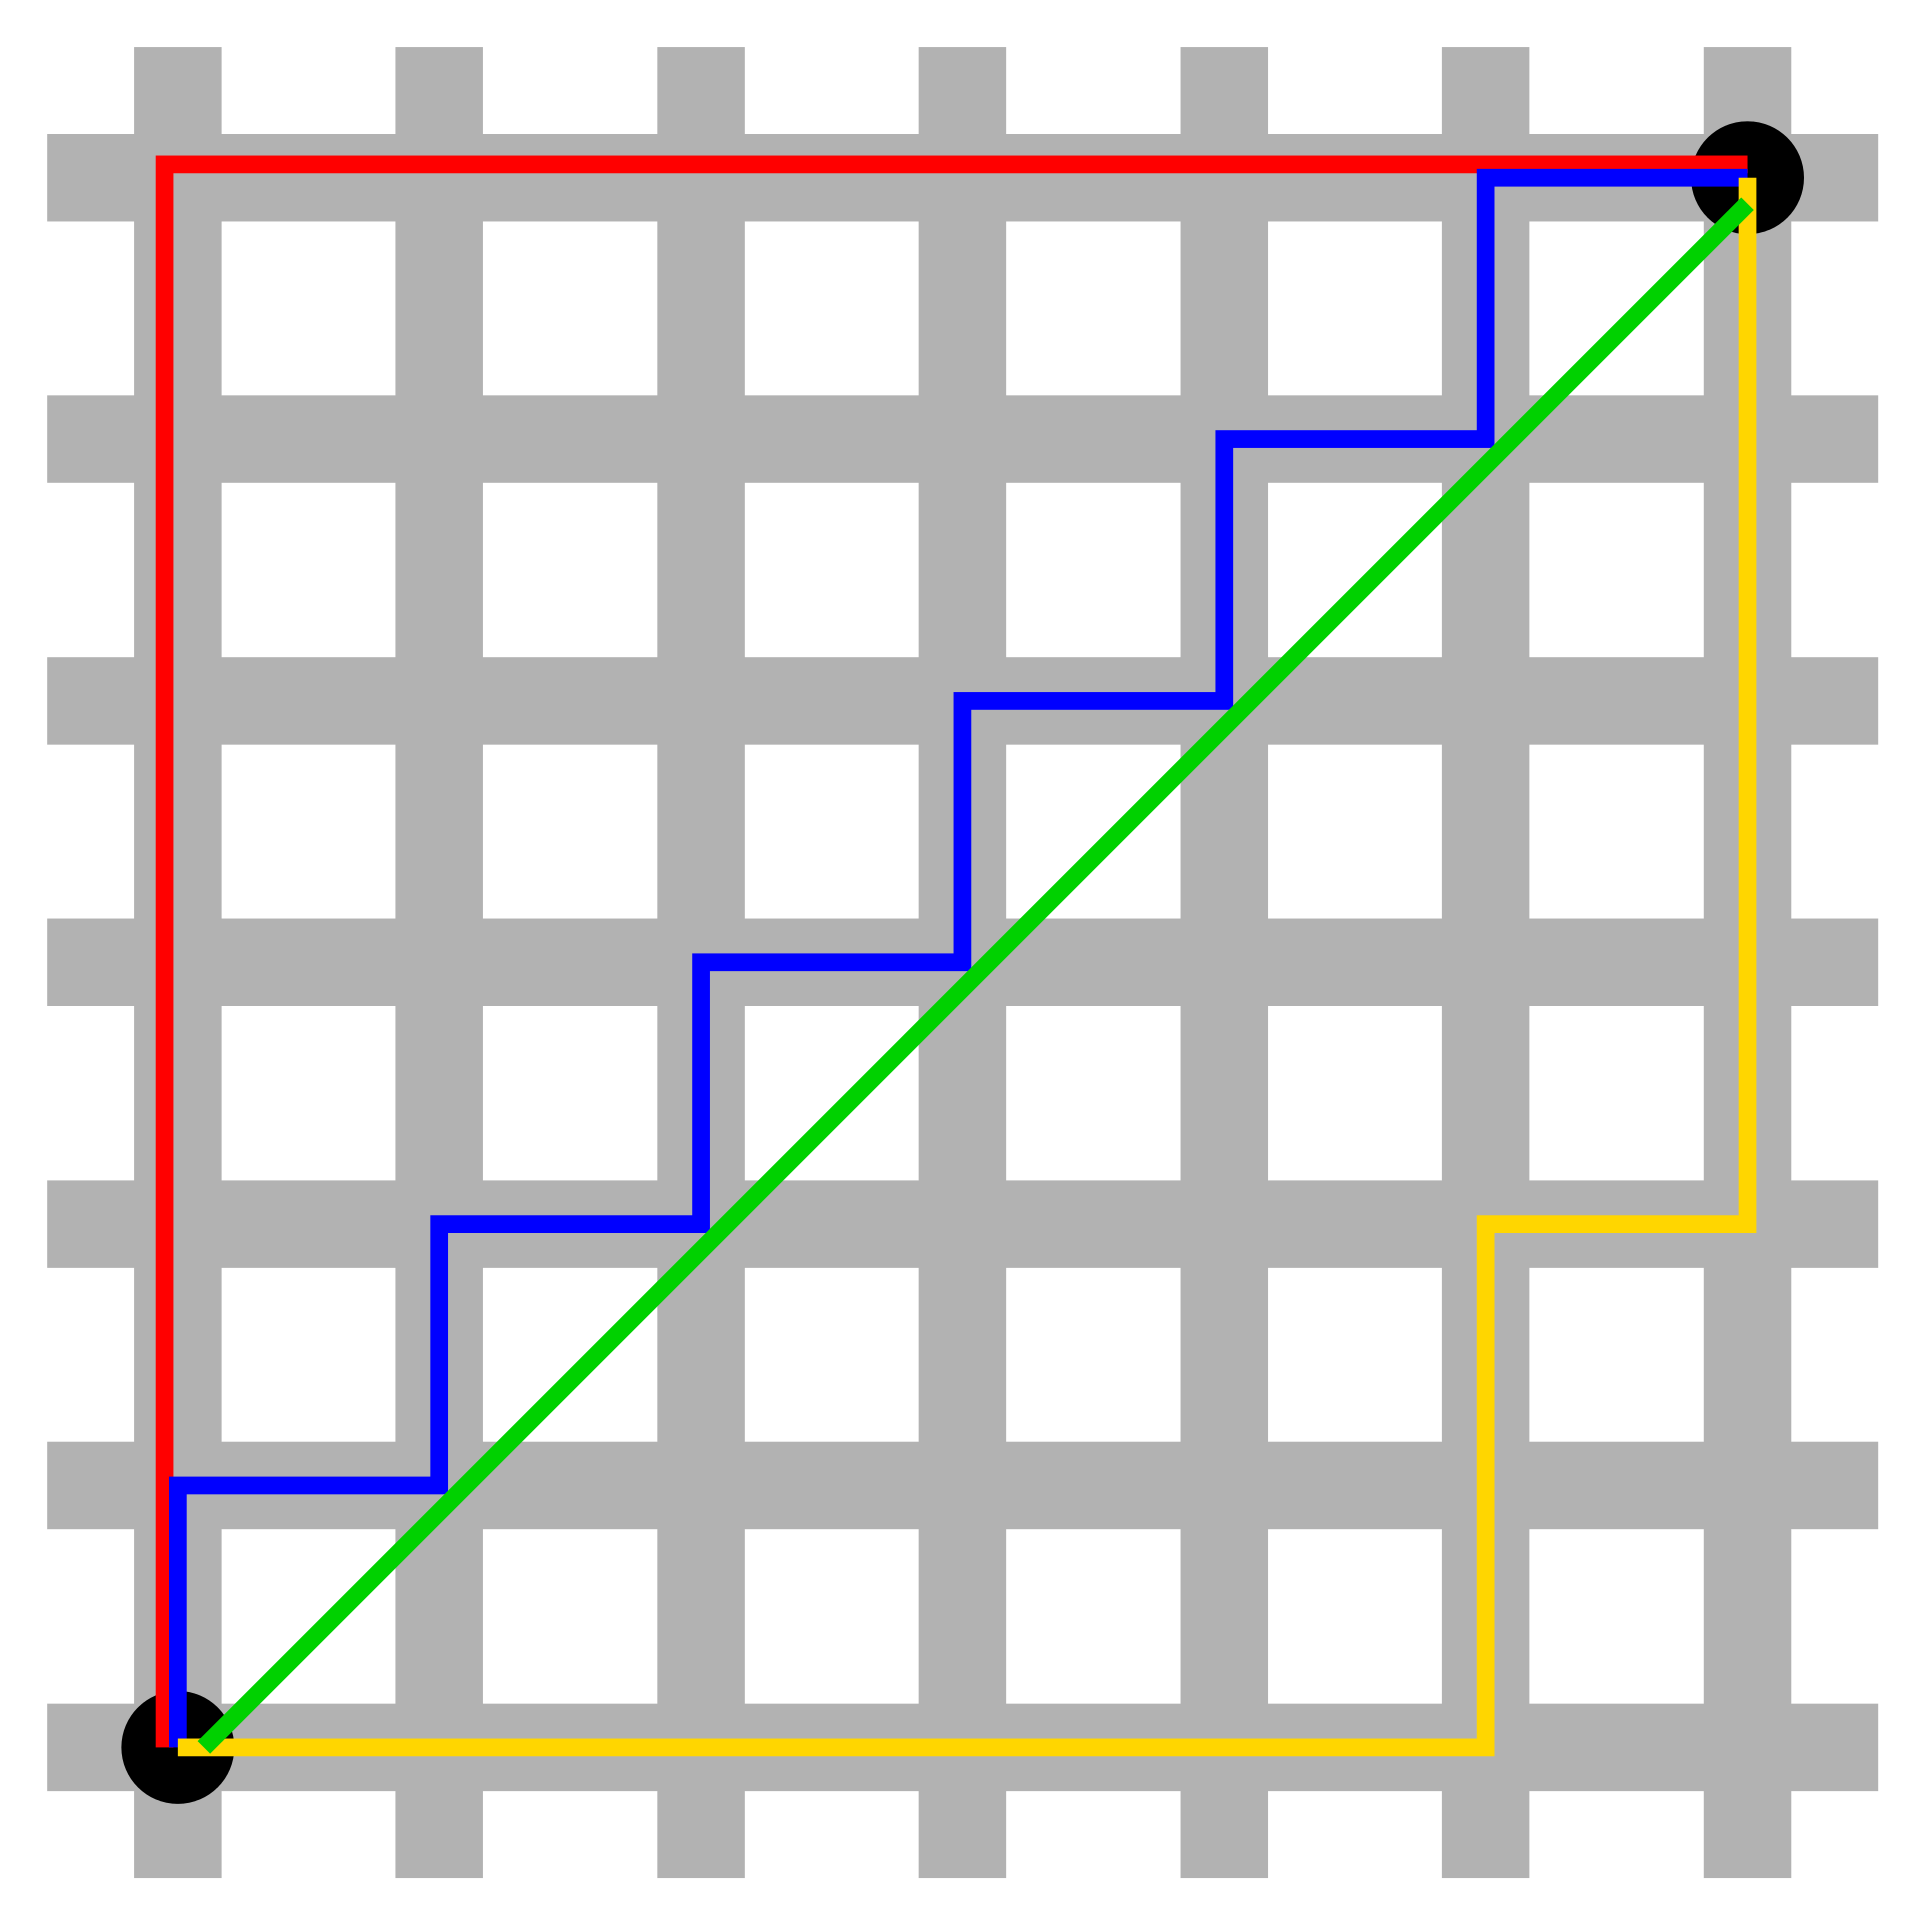
\includegraphics[scale=0.1]{images/Manhattan_distance.svg.png}
            \caption{A picture description of Manhattan distance}
        \end{figure}
        \item \underline{Euclidean distance}: $$d_2(x,y)=\sqrt{|x_1-y_1|^2+ \cdots |x_n - y_n|^2}$$
        The first and the second properties are clear. For the third property, it follows by Pythagoras theorem or Cauchy-Schwarz inequality.
        \item \underline{Chebyshev distance}: $$d_{\infty}(x,y)=sup\{|x_1-y_1|,\cdots ,|x_n-y_n|\}$$
    \end{itemize}
\end{definition}



\begin{lemma} \label{sup2eq}
    In $\R^n$ with the previous norms, we have
    $$\lVert x \rVert_{\infty} \leq \lVert x \rVert_2 \leq \sqrt{n} \lVert x \rVert_{\infty}$$
\end{lemma}


\begin{lemma} \label{21eq}
    In $\R^n$ with the previous norms, we have
    $$\lVert x \rVert_2 \leq \lVert x \rVert_1 \leq \sqrt{n} \lVert x \rVert_2$$
\end{lemma}

\begin{definition}
    In $\R^n$, let $a \in \R^n$ be arbitrary
\begin{itemize}
    \item the \underline{open cube} is $$C(a,\epsilon)=\{x \in \R^n: \lVert x-a \rVert_{\infty}<\epsilon\}$$
    \item the \underline{usual open ball} is just $$B(a;\epsilon)=\{x \in \R^n:  \lVert x-a \rVert_2<\epsilon\}$$
    \item the \underline{taxicab ball} i.e.manhattan ball is defined as $$T(a;\epsilon)=\{x \in \R^n:  \lVert x-a \rVert_1<\epsilon\}$$
\end{itemize}
\begin{figure}[h]
    \centering
    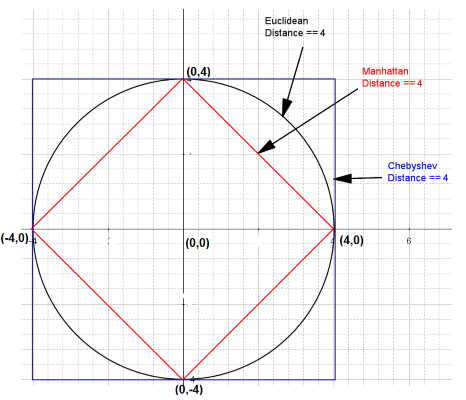
\includegraphics[scale=0.5]{images/FSnE9ZFXoAkp2Tp.png}
    \caption{Ball of radius 4 of the previous distance functions}
\end{figure}
\end{definition}

\begin{lemma}\label{CcontainsB}
    $$B(a;\epsilon) \subset C(a;\epsilon) \subset B(a;\sqrt{n}\epsilon)$$
\end{lemma}


\begin{lemma}
    $$T(a;\epsilon) \subset B(a;\epsilon) \subset T(a;\sqrt{n}\epsilon)$$
\end{lemma}

\begin{definition}
    Let $V$ be a vector space. Given $\lVert \cdot \rVert_a$ and $\lVert \cdot \rVert_b$ two norms on the vector space, we say $\lVert \cdot \rVert_a$ and $\lVert \cdot \rVert_b$ are \underline{equivalent} if there 
    exist positive constants $r_1,r_2$ such that for all $v \in V$ we have 
    $$r_1 \lVert x \rVert_a \leq \lVert x \rVert_b \leq r_2\lVert x \rVert_a$$
\end{definition}

\begin{theorem}
    $\lVert \cdot \rVert_1$ and $\lVert \cdot \rVert_2$ and $\lVert \cdot \rVert_{\infty}$ are equivalent.
\end{theorem}


\begin{theorem*}
    If the vector space is a finite-dimensional real or complex one, all norms are equivalent.
\end{theorem*}

\begin{theorem*} \label{topology induced by eq norms}
    The topologies induced by two equivalent norms are the same.
\end{theorem*}
\noindent \textbf{Remark}:
\begin{itemize}
    \item We are not going to prove this theorem right now, this only gives an intuition of why we study metric topology.
\end{itemize}

\section{Metric Topology}
We now know that the three norms defined on $\R^n$ will induce the same topology on $\R^n$. 
So the three different norms derive three different metric spaces. And the three metric spaces will have the same structure. 
In this chapter, we focus on the structure of $\R^n$, i.e. the topology of $\R^n$. Actually, we can start from any of the three metric spaces(usually we pick the Euclidean norm) to study the structure of $\R^n$.
Therefore the most important thing for now is to learn how to analyze the structure of the general metric space.
\begin{definition}
    Given any metric space $(X,d)$, an \underline{open set} is a subset $A \subset X$ such that $$\forall a \in A. \exists \epsilon >0. U(a;\epsilon) \subset A$$
\end{definition}
\noindent \textbf{Examples}:
\begin{itemize}
    \item The interval $(a,b)$ in $\R$ is an open set.
    \item The interval $(a,b]$ in $\R$ is not an open set because of the point $b$.
    \item $\bigcup_{n \geq 1}^{\infty}(\frac{1}{2^{n+1}},\frac{1}{2^n})$ is open.
    \item $\bigcap_{n \geq 1}^{\infty}(-\frac{1}{n},\frac{1}{n})=\{0\}$ is not an open set.
\end{itemize}
\noindent \textbf{Remark}:
\begin{itemize}
    \item An arbitrary union of open sets is open.
    \item A finite intersection of open sets is open.
    \item Can check that $\mathcal{B}_d=\{B(x;\epsilon):x\in X\text{ and }\epsilon>0\}$ can form a basis for $X$.
\end{itemize}

\begin{definition}
    Given a set $X$ and a metric $d$, The topology generated by the basis $\mathcal{B}_d=\{B(x;\epsilon):x\in X\text{ and }\epsilon>0\}$ is called the \underline{metric topology}.
\end{definition}

\begin{definition}
    If $U$ is any open set containing $x_0$, we commonly refer to U simply as a \underline{neighborhood of $x_0$}.
\end{definition}

\begin{definition}
    A set is closed if and only if it's complement is open.
\end{definition}
\noindent \textbf{Remark}:
\begin{itemize}
    \item Any intersection of closed sets is close.
    \item Finite union of closed sets is close.
\end{itemize}

\begin{lemma}
    Let $(X,d)$ be a metric space, let $Y \subset X$. Then 
    $$A \subset Y \text{ is open in }Y \Longrightarrow A=Y\cap U \text{ for some open }U \text{ in }X.$$
\end{lemma}


\begin{definition}
    Given any subset $A \subset X$, a point $x \in A$ is a \underline{limit point} of $A$ if 
    $$\forall \epsilon >0. \exists x' \in A. x' \neq x \text{ and }x' \in U(x;\epsilon)$$
\end{definition}
\noindent \textbf{Example}:
\begin{itemize}
    \item For the interval $[0,1)$, 0 is a limit point and 1 is a limit point.
\end{itemize}
\noindent \textbf{Remark}:
\begin{itemize}
    \item In any metric space $(X,d)$ with the metric topology, if $x_0$ is a limit point of $Y \subset X$, then
    $$\forall \epsilon >0. \exists \text{ infinitely many }x_1 \in U(x_0;\epsilon). x_1 \in Y$$
    \underline{A finite set in metric space has no limit points.}\\
    Because each point $p$ has a positive distance to the points of the set (other than itself if it is a member of the set), 
    and since there are finitely many of them, there is a minimum distance $d$. The open ball of radius $d$ around $p$ doesn't contain any elements of the set other than $p$.
    \item The statement is not true when we generalize to topological spaces. 
    For example, $$X=\{1,2,3\}, \mathcal{T}=\{\emptyset,\{1,2\},\{1,3\},\{2,3\},\{1,2,3\}\}$$
    the set $\{1,2\}$ has limit point 3.
\end{itemize}

\begin{theorem}
    A set $A \subset X$ is closed if and only if it contains all it's limit points.
\end{theorem}

\begin{definition}
    Let $(X,d)$ be a metric space, let $A \subset X$, we define the \underline{closure} of $A$:
    $$\overline{A}=A \cup \{\text{all limit points of } A\}$$
\end{definition}

\begin{lemma}
    $$\overline{A}=\bigcap \{\text{closed sets containing $A$}\}$$
\end{lemma}

\begin{definition}
    Given any set $A \subset X$, the \underline{interior} of $A$ is 
    $$Int(A)=\bigcup \{\text{all open sets contained in $A$}\}$$
\end{definition}

\begin{definition}
    Given any set $A \subset X$, the \underline{exterior} of $A$ is 
    $$Ext(A)=\bigcup \{\text{all open sets contained in $A^C$}\}$$
\end{definition}

\begin{definition}
    Given any set $A \subset X$, the \underline{boundary} of $A$ is 
    $$Bd(A)= X\setminus(Int(A) \cup Ext(A))$$ 
    some books will use the notation $\partial A$.
\end{definition}

\section{Continuity in Metric Space}

\begin{definition}
    Let $(X,d),(Y,h)$ be metric spaces. Construct a function $f:X \longrightarrow Y$ over a subset $A \subset X$. 
    $$f:A \longrightarrow Y$$
    Let $x_0 \in A$, we say $f$ is \underline{continuous at $x_0$} iff 
    $$\forall \text{open $V \subset Y$ containing $f(x_0)$ }. \exists \text{open }U \subset X \text{ containing }x_0. f(U) \subset V $$
    We can use $\epsilon - \delta$ language to express the definition clearly:
    \begin{itemize}
        \item $\forall \epsilon>0. \exists \delta >0. \forall x \in A. x \in U(x_0;\delta) \Longrightarrow f(x) \in V(f(x_0);\epsilon)$ where $V$ is open ball in $(Y,h)$.
        \item $\forall \epsilon>0. \exists \delta >0. \forall x \in A. d(x;x_0)<\delta \Longrightarrow h(f(x);f(x_0))<\epsilon$.
    \end{itemize}
\end{definition}

\begin{definition}
    We say $f$ is \underline{continuous} if it is continuous at each point $x_0$ of $A$.
\end{definition}

\begin{theorem}
    A map $f:(X,d) \longrightarrow (Y,h)$ is continuous if and only if the preimage of every open subset is open.
    $$\forall V \subset Y \text{ open. } f^{-1}(V) \text{ is open in }X$$
\end{theorem}


\noindent \textbf{Examples}:
\begin{itemize}
    \item Let $X=\R^3$, $Y$ be any set. $A=\{(0,0,0),(0,\sqrt{2},-\sqrt{3}),(e,\pi,e^{\pi})\}$,\\ then $f:A \longrightarrow Y$ is continuous.\\
    First, we claim that \underline{any subset of $A$ is open}.
    \begin{proof}
        Let $x_0 \in A$ be arbitrary, $x_0$ is the only element in $\{x_0\}$. 
        Let $\epsilon=min\{d(x_0,x_1),d(x_0,x_2)\}$, then $U(x_0,\epsilon)=\{x_0\} \subset \{x_0\}$. 
        So $\{x_0\}$ is open. Any subset of $A$ is the union of singletons, hence is open.
    \end{proof}
    Fix $x_0$, let $U \subset Y$ be an open set that contains $f(x_0)$. 
    By the claim above, $f^{-1}(U)$ is open. So $f$ is indeed continuous. 
    More generally, if $A$ is finite, then $f:A \longrightarrow Y$ is continuous.
    \item Let $A=\overline{U(x_0,1)}\cup \{p_1,\cdots,p_n\}$ with all $p_i \notin \overline{U(x_0;1)}$\\
    Suppose $f:\overline{U(x_0;1)} \longrightarrow Y$ is continuous, then $f:A \longrightarrow Y$ is continuous.\\
    \underline{In MAT157, we knew that $f$ is continuous on isolated points.}
\end{itemize}

\begin{theorem} \label{dist continuous}
    Let $(X,d)$ be a metric space, fix a subset $C$ in the metric space $X$.
    Then the function $$dist:X \longrightarrow \R$$ is continuous.
\end{theorem}

\begin{definition}
    $f:(X,d) \longrightarrow (Y,h)$ is \underline{uniformly continuous} if 
    $$\forall \epsilon >0. \exists \delta >0. \forall x,y \in X.d(x,y)<\delta \Longrightarrow h(f(x),f(y))<\epsilon$$
\end{definition}
\noindent \textbf{Examples}: functions which are continuous but not uniformly continuous.
\begin{itemize}
    \item $f:[0,\infty) \longrightarrow \R,f(x)=x^2$
    \item $f:(0,1) \longrightarrow \R,f(x)=\frac{1}{x}$
\end{itemize}

\section{Compactness in Metric Space}

\begin{definition}
    Let $(X,d)$ be a metric space, $Y \subset X$ ,an \underline{open cover} of $Y$ is a collection of open sets $U_\alpha,\alpha \in A$, such that $$Y \subset \bigcup_{\alpha \in A}U_{\alpha}$$
\end{definition}

\begin{definition}
    Let $(X,d)$ be a metric space, a subset $Y \subset X$ is \underline{compact} if any open cover of $Y$ has a finite subcover.
    Suppose $U_{\alpha},\alpha \in A$ is an open cover of $Y$, $Y$ is compact if there exists a finite collection $\alpha_1,\cdots,\alpha_n \in A$ such that $$Y \subset \bigcup_{i=1}^n U_{\alpha_i}$$
\end{definition}
\noindent \textbf{Example}:
\begin{itemize}
    \item In $\R$, the interval $[a,b]$ is compact.
\end{itemize}

\begin{theorem}
    Every closed subspace of a compact space is compact.
\end{theorem}

\begin{theorem}\label{compactimpliesclosedbounded}
    If $Y \subset (X,d)$ is compact, then $Y$ is closed and bounded.
\end{theorem}

\begin{theorem} \label{lemmaevt}
    Let $f:(X,d) \longrightarrow (Y,h)$ be a continuous function. If $A$ is compact in $X$, then $f(A)$ is compact in $Y$.
\end{theorem}

\begin{corollary}[Extreme Value Theorem] \label{evt}
    Let $f:A \subset X \longrightarrow \R$ be a continuous function. If $A$ is compact, then $f(A)$ has a maximum value and a minimum value.
\end{corollary}

\begin{theorem}[The $\epsilon$-neighborhood Theorem] \label{epsilon neighborhood thm}
    Let $(X,d)$ be a metric space, consider a compact set $Y \subset X$ and an open set $U$ containing $Y$. 
    Then there exists $\epsilon>0$ such that an $epsilon$-neighborhood of $Y$ is contained in $U$.
\end{theorem}

\begin{theorem}\label{continuous function on compact set is uniformly continuous}
    If $(X,d)$ and $(Y,h)$ be metric spaces, let $X$ be compact and $f:X \longrightarrow Y$ continuous. 
    Then $f$ is uniformly continuous.
\end{theorem}



\begin{theorem}\label{rectanglecompact}
    The rectangle $Q=[a_1,b_1]\times \cdots \times [a_n,b_n] \subset \R^n$ is compact.
\end{theorem}


\begin{definition}
    a topological space X is \underline{sequentially compact} if every sequence of points in $X$ has a convergent subsequence converging to a point in $X$.
\end{definition}

\begin{theorem}
    In metric space, compactness is equivalent to sequentially compactness.
\end{theorem}

\section{Connectedness in  Metric Space}

\begin{definition}
    Let $(X,d)$ be a metric space, we say $X$ is \underline{connected} if $X$ cannot be written as the union of two disjoint non-empty sets $A$ and $B$, each of which is open in $X$.
\end{definition}

\begin{theorem}
    The real line $\R$ is connected and so are the intervals and rays.
\end{theorem}

\begin{theorem}
    Let $(X,d)$ be a connected metric space, if $f:X \longrightarrow Y$ is continuous, then $f(X)$ is connected in $Y$.
\end{theorem}

\begin{corollary}[Intermediate-Value Theorem]
    Let $(X,d)$ be a metric space and $f:X \longrightarrow \R$ is continuous, then if $f(x_0) < r < f(x_1)$ for some points $x_0,x_1$ of $X$,then $f(x)=r$ for some point $x$ of $X$.
\end{corollary}

\begin{definition}
    Let $a,b$ be two points in $\R^n$, the \underline{line segment} joining $a$ and $b$ is:
    $$\{a+t(b-a): t\in [0,1]\}$$
\end{definition}
\begin{figure}[ht]
    \centering
    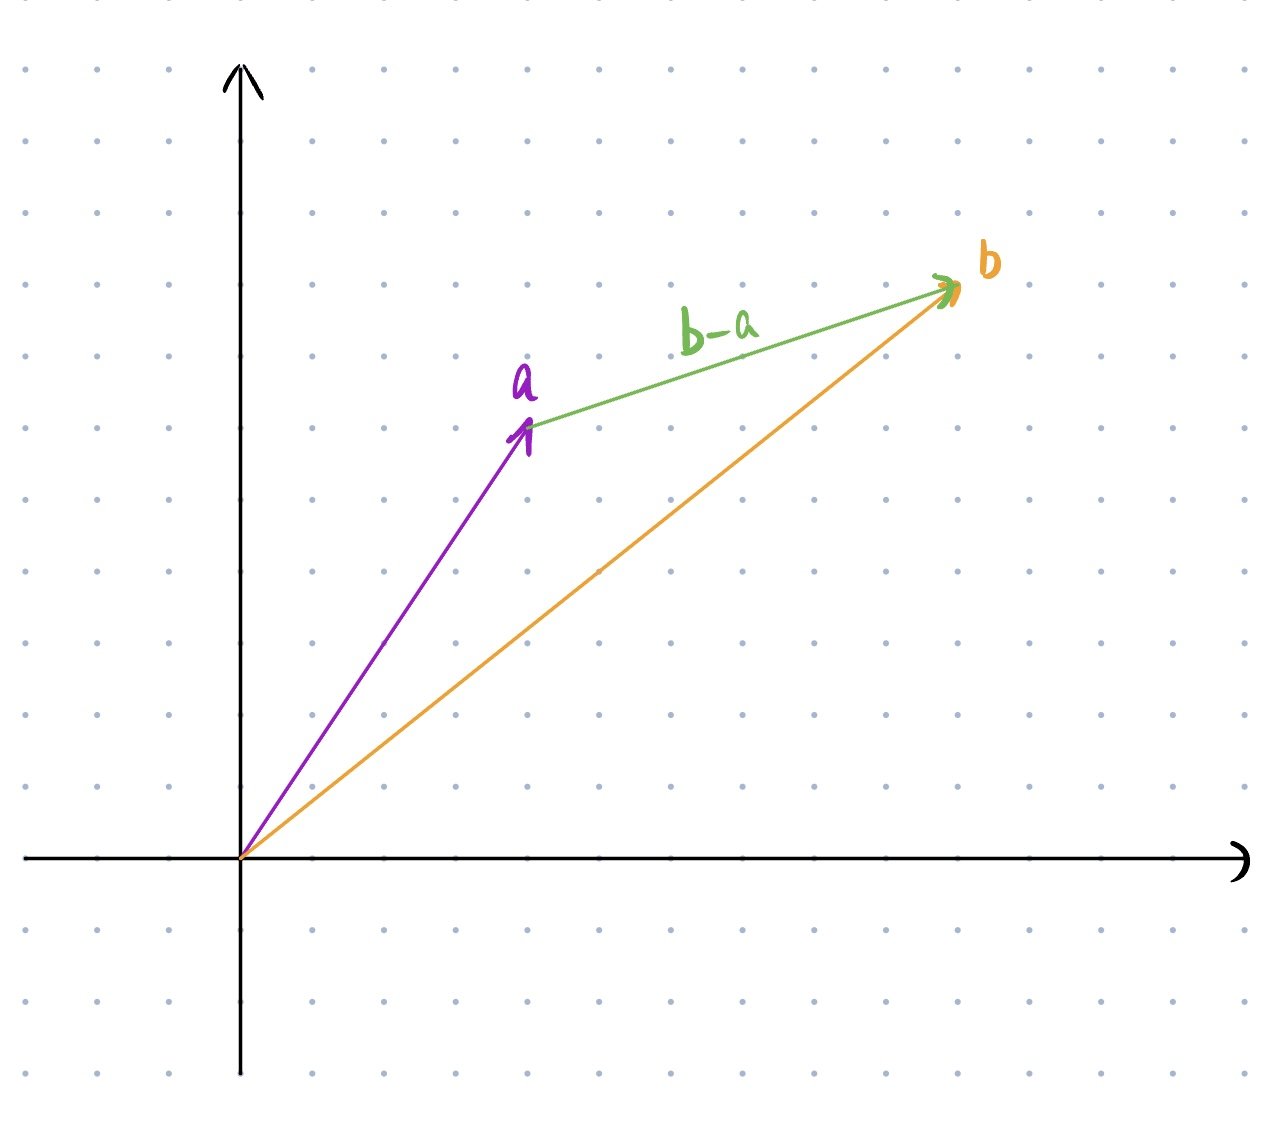
\includegraphics[scale=0.17]{images/line_segment.jpg}
    \caption{the line segment joining a and b}
\end{figure}

\begin{definition}
    A subset $A \subset \R^n$ is \underline{convex} if $\forall a,b \in A$, the line segment joining $a$ and $b$ is contained in $A$.
\end{definition}

\begin{theorem}
    Open balls and open cubes in $\R^n$ are convex.
\end{theorem}

\begin{theorem}
    Open rectangles and closed rectangles in $\R^n$ are convex.
\end{theorem}